%% For double-blind review submission, w/o CCS and ACM Reference (max submission space)
\documentclass[10pt, sigplan]{acmart}
%%\settopmatter{printfolios=true,printccs=false,printacmref=false}
%% For double-blind review submission, w/ CCS and ACM Reference
%\documentclass[sigplan,10pt,review,anonymous]{acmart}\settopmatter{printfolios=true}
%% For single-blind review submission, w/o CCS and ACM Reference (max submission space)
%\documentclass[sigplan,10pt,review]{acmart}\settopmatter{printfolios=true,printccs=false,printacmref=false}
%% For single-blind review submission, w/ CCS and ACM Reference
%\documentclass[sigplan,10pt,review]{acmart}\settopmatter{printfolios=true}
%% For final camera-ready submission, w/ required CCS and ACM Reference
%\documentclass[sigplan,10pt]{acmart}\settopmatter{}


%% Conference information
%% Supplied to authors by publisher for camera-ready submission;
%% use defaults for review submission.
%\acmConference[PL'17]{ACM SIGPLAN Conference on Programming Languages}{January 01--03, 2017}{New York, NY, USA}
%\acmYear{2017}
%\acmISBN{} % \acmISBN{978-x-xxxx-xxxx-x/YY/MM}
%\acmDOI{} % \acmDOI{10.1145/nnnnnnn.nnnnnnn}
%\startPage{1}

%% Copyright information
%% Supplied to authors (based on authors' rights management selection;
%% see authors.acm.org) by publisher for camera-ready submission;
%% use 'none' for review submission.
\setcopyright{none}
%\setcopyright{acmcopyright}
%\setcopyright{acmlicensed}
%\setcopyright{rightsretained}
%\copyrightyear{2017}           %% If different from \acmYear

%% Bibliography style

%\bibliographystyle{ACM-Reference-Format}

%% Citation style
%\citestyle{acmauthoryear}  %% For author/year citations
\citestyle{acmnumeric}     %% For numeric citations
%\setcitestyle{nosort}      %% With 'acmnumeric', to disable automatic
                            %% sorting of references within a single citation;
                            %% e.g., \cite{Smith99,Carpenter05,Baker12}
                            %% rendered as [14,5,2] rather than [2,5,14].
%\setcitesyle{nocompress}   %% With 'acmnumeric', to disable automatic
                            %% compression of sequential references within a
                            %% single citation;
                            %% e.g., \cite{Baker12,Baker14,Baker16}
                            %% rendered as [2,3,4] rather than [2-4].


%%%%%%%%%%%%%%%%%%%%%%%%%%%%%%%%%%%%%%%%%%%%%%%%%%%%%%%%%%%%%%%%%%%%%%
%% Note: Authors migrating a paper from traditional SIGPLAN
%% proceedings format to PACMPL format must update the
%% '\documentclass' and topmatter commands above; see
%% 'acmart-pacmpl-template.tex'.
%%%%%%%%%%%%%%%%%%%%%%%%%%%%%%%%%%%%%%%%%%%%%%%%%%%%%%%%%%%%%%%%%%%%%%


%% Some recommended packages.
\usepackage{booktabs}   %% For formal tables:
                        %% http://ctan.org/pkg/booktabs
\usepackage{subcaption} %% For complex figures with subfigures/subcaptions
                        %% http://ctan.org/pkg/subcaption
\usepackage{xspace}
\usepackage{graphicx}
\usepackage{ifthen}
\usepackage{pgfplots}
\usepackage{listings}
\usepackage{multirow}
\usepgfplotslibrary{statistics}
\usepackage{dblfloatfix} %enable fig at bottom of page
%



% Source Code
%\usepackage{color}
%\usepackage{textcomp}
%\usepackage{listings}
%\usepackage{ulem}
%\usepackage[T1]{fontenc}
%\usepackage{times}
% \usepackage{needspace}
 

% Source Code
\usepackage{color}
\usepackage{textcomp}
\usepackage{listings}

\definecolor{source}{gray}{0.85}% my comment style
\newcommand{\myCommentStyle}[1]{{\footnotesize\sffamily\color{gray!100!white} #1}}
%\newcommand{\myCommentStyle}[1]{{\footnotesize\sffamily\color{black!100!white} #1}}

% my string style
\newcommand{\myStringStyle}[1]{{\footnotesize\sffamily\color{violet!100!black} #1}}
%\newcommand{\myStringStyle}[1]{{\footnotesize\sffamily\color{black!100!black} #1}}

% my symbol style
\newcommand{\mySymbolStyle}[1]{{\footnotesize\sffamily\color{violet!100!black} #1}}
%\newcommand{\mySymbolStyle}[1]{{\footnotesize\sffamily\color{black!100!black} #1}}

% my keyword style
\newcommand{\myKeywordStyle}[1]{{\footnotesize\sffamily\color{green!70!black} #1}}
%\newcommand{\myKeywordStyle}[1]{{\footnotesize\sffamily\color{black!70!black} #1}}

% my global style
\newcommand{\myGlobalStyle}[1]{{\footnotesize\sffamily\color{blue!100!black} #1}}
%\newcommand{\myGlobalStyle}[1]{{\footnotesize\sffamily\color{black!100!black} #1}}

% my number style
\newcommand{\myNumberStyle}[1]{{\footnotesize\sffamily\color{brown!100!black} #1}}
%\newcommand{\myNumberStyle}[1]{{\footnotesize\sffamily\color{black!100!black} #1}}

\lstset{
language={},
% characters
tabsize=3,
escapechar={!},
keepspaces=true,
breaklines=true,
alsoletter={\#},
literate={\$}{{{\$}}}1,
breakautoindent=true,
columns=fullflexible,
showstringspaces=false,
% background
frame=single,
aboveskip=1em, % automatic space before
framerule=0pt,
basicstyle=\footnotesize\sffamily\color{black},
keywordstyle=\myKeywordStyle,% keyword style
commentstyle=\myCommentStyle,% comment style
frame=single,%
backgroundcolor=\color{source},
% numbering
stepnumber=1,
numbersep=10pt,
numberstyle=\tiny,
numberfirstline=true,
% caption
captionpos=b,
% formatting (html)
moredelim=[is][\bfseries]{<b>}{</b>},
moredelim=[is][\textit]{<i>}{</i>},
moredelim=[is][\underbar]{<u>}{</u>},
moredelim=[is][\color{red}\uwave]{<wave>}{</wave>},
moredelim=[is][\color{red}\sout]{<del>}{</del>},
moredelim=[is][\color{blue}\underbar]{<ins>}{</ins>},
% smalltalk stuff
morecomment=[s][\myCommentStyle]{"}{"},
%    morecomment=[s][\myvs]{|}{|},
morestring=[b][\myStringStyle]',
moredelim=[is][]{<sel>}{</sel>},
moredelim=[is][]{<rcv>}{</rcv>},
moredelim=[is][\itshape]{<symb>}{</symb>},
moredelim=[is][\scshape]{<class>}{</class>},
morekeywords={true,false,nil,self,super,thisContext},
identifierstyle=\idstyle,
}

\makeatletter
\newcommand*\idstyle[1]{%
\expandafter\id@style\the\lst@token{#1}\relax%
}
\def\id@style#1#2\relax{%
\ifnum\pdfstrcmp{#1}{\#}=0%
% this is a symbol
\mySymbolStyle{\the\lst@token}%
\else%
\edef\tempa{\uccode`#1}%
\edef\tempb{`#1}%
\ifnum\tempa=\tempb%
% this is a global
\myGlobalStyle{\the\lst@token}%
\else%
\the\lst@token%
\fi%
\fi%
}
\makeatother


%\newcommand{\ct}{\lstinline[backgroundcolor=\color{white}]}
%\newcommand{\needlines}[1]{\Needspace{#1\baselineskip}}
\newcommand{\lct}{\texttt}

\lstnewenvironment{code}{%
    \lstset{%
    % frame=lines,
    frame=single,
    framerule=0pt,
    mathescape=false
    }%
    \noindent%
    \minipage{\linewidth}%
}{%
    \endminipage%
}%


\lstnewenvironment{codeWithLineNumbers}{%
    \lstset{%
    % frame=lines,
    frame=single,
    framerule=0pt,
    mathescape=false,
    numbers=left
    }%
    \noindent%
    \minipage{\linewidth}%
}{%
    \endminipage%
}%



\newenvironment{codeNonSmalltalk}
{\begin{alltt}\sffamily}
{\end{alltt}\normalsize}



\usepackage{xcolor}
\newcommand{\todo}[1]{\color{orange}\fbox{\bfseries\sffamily\scriptsize TODO:}{\sf\small$\blacktriangleright$\textit{#1}$\blacktriangleleft$}\color{black}}
\newcommand{\sd}[1]{\color{red}\fbox{\bfseries\sffamily\scriptsize Stef:}{\sf\small$\blacktriangleright$\textit{#1}$\blacktriangleleft$}\color{black}}
\newcommand{\sk}[1]{\color{blue}\fbox{\bfseries\sffamily\scriptsize Sophie:}{\sf\small$\blacktriangleright$\textit{#1}$\blacktriangleleft$}\color{black}}
\newcommand{\cba}[1]{\color{purple}\fbox{\bfseries\sffamily\scriptsize Clement:}{\sf\small$\blacktriangleright$\textit{#1}$\blacktriangleleft$}\color{black}}
%\newcommand*{rotatebox{75}}




% Source Code
%\usepackage{color}
%\usepackage{textcomp}
%\usepackage{listings}
%\usepackage{ulem}
%\usepackage[T1]{fontenc}
%\usepackage{times}
% \usepackage{needspace}
 

% Source Code
\usepackage{color}
\usepackage{textcomp}
\usepackage{listings}

\definecolor{source}{gray}{0.85}% my comment style
\newcommand{\myCommentStyle}[1]{{\footnotesize\sffamily\color{gray!100!white} #1}}
%\newcommand{\myCommentStyle}[1]{{\footnotesize\sffamily\color{black!100!white} #1}}

% my string style
\newcommand{\myStringStyle}[1]{{\footnotesize\sffamily\color{violet!100!black} #1}}
%\newcommand{\myStringStyle}[1]{{\footnotesize\sffamily\color{black!100!black} #1}}

% my symbol style
\newcommand{\mySymbolStyle}[1]{{\footnotesize\sffamily\color{violet!100!black} #1}}
%\newcommand{\mySymbolStyle}[1]{{\footnotesize\sffamily\color{black!100!black} #1}}

% my keyword style
\newcommand{\myKeywordStyle}[1]{{\footnotesize\sffamily\color{green!70!black} #1}}
%\newcommand{\myKeywordStyle}[1]{{\footnotesize\sffamily\color{black!70!black} #1}}

% my global style
\newcommand{\myGlobalStyle}[1]{{\footnotesize\sffamily\color{blue!100!black} #1}}
%\newcommand{\myGlobalStyle}[1]{{\footnotesize\sffamily\color{black!100!black} #1}}

% my number style
\newcommand{\myNumberStyle}[1]{{\footnotesize\sffamily\color{brown!100!black} #1}}
%\newcommand{\myNumberStyle}[1]{{\footnotesize\sffamily\color{black!100!black} #1}}

\lstset{
language={},
% characters
tabsize=3,
escapechar={!},
keepspaces=true,
breaklines=true,
alsoletter={\#},
literate={\$}{{{\$}}}1,
breakautoindent=true,
columns=fullflexible,
showstringspaces=false,
% background
frame=single,
aboveskip=1em, % automatic space before
framerule=0pt,
basicstyle=\footnotesize\sffamily\color{black},
keywordstyle=\myKeywordStyle,% keyword style
commentstyle=\myCommentStyle,% comment style
frame=single,%
backgroundcolor=\color{source},
% numbering
stepnumber=1,
numbersep=10pt,
numberstyle=\tiny,
numberfirstline=true,
% caption
captionpos=b,
% formatting (html)
moredelim=[is][\bfseries]{<b>}{</b>},
moredelim=[is][\textit]{<i>}{</i>},
moredelim=[is][\underbar]{<u>}{</u>},
moredelim=[is][\color{red}\uwave]{<wave>}{</wave>},
moredelim=[is][\color{red}\sout]{<del>}{</del>},
moredelim=[is][\color{blue}\underbar]{<ins>}{</ins>},
% smalltalk stuff
morecomment=[s][\myCommentStyle]{"}{"},
%    morecomment=[s][\myvs]{|}{|},
morestring=[b][\myStringStyle]',
moredelim=[is][]{<sel>}{</sel>},
moredelim=[is][]{<rcv>}{</rcv>},
moredelim=[is][\itshape]{<symb>}{</symb>},
moredelim=[is][\scshape]{<class>}{</class>},
morekeywords={true,false,nil,self,super,thisContext},
identifierstyle=\idstyle,
}

\makeatletter
\newcommand*\idstyle[1]{%
\expandafter\id@style\the\lst@token{#1}\relax%
}
\def\id@style#1#2\relax{%
\ifnum\pdfstrcmp{#1}{\#}=0%
% this is a symbol
\mySymbolStyle{\the\lst@token}%
\else%
\edef\tempa{\uccode`#1}%
\edef\tempb{`#1}%
\ifnum\tempa=\tempb%
% this is a global
\myGlobalStyle{\the\lst@token}%
\else%
\the\lst@token%
\fi%
\fi%
}
\makeatother


%\newcommand{\ct}{\lstinline[backgroundcolor=\color{white}]}
%\newcommand{\needlines}[1]{\Needspace{#1\baselineskip}}
\newcommand{\lct}{\texttt}

\lstnewenvironment{code}{%
    \lstset{%
    % frame=lines,
    frame=single,
    framerule=0pt,
    mathescape=false
    }%
    \noindent%
    \minipage{\linewidth}%
}{%
    \endminipage%
}%


\lstnewenvironment{codeWithLineNumbers}{%
    \lstset{%
    % frame=lines,
    frame=single,
    framerule=0pt,
    mathescape=false,
    numbers=left
    }%
    \noindent%
    \minipage{\linewidth}%
}{%
    \endminipage%
}%



\newenvironment{codeNonSmalltalk}
{\begin{alltt}\sffamily}
{\end{alltt}\normalsize}



\begin{document}

%% Title information
\title[Assessing primitives performance on multi-stage execution]{Assessing primitives performance\\ on multi-stage execution}

%% Author with single affiliation.
\author{Sophie Kaleba}
                                        %% can be repeated if necessary
\affiliation{
  %\position{Position1}
  \department{RMoD}              %% \department is recommended
  \institution{Inria}            %% \institution is required
 % \streetaddress{Street1 Address1}
  \city{Lille}
  %\state{France}
  %\postcode{Post-Code1}
  \country{France}                    %% \country is recommended
}
\email{sophie.kaleba@etudiant.univ-lille1.fr}          %% \email is recommended

%% Author with two affiliations and emails.
\author{Cl\'ement B\'era}
\affiliation{
  % \position{}
	\department{Software Languages Lab}              %% \department is recommended
	\institution{Vrije Universiteit Brussel}            %% \institution is required
	\city{Brussel}
  % \state{}
  % \postcode{}
	\country{Belgium}                    %% \country is recommended
}
\email{clement.bera@vub.ac.be}          %% \email is recommended

%% Author with two affiliations and emails.
\author{St\'ephane Ducasse}
\affiliation{
 % \position{Position2b}
  \department{RMoD}             %% \department is recommended
  \institution{Inria}           %% \institution is required
  %\streetaddress{Street3b Address2b}
  \city{Lille}
  %\state{State2b}
  %\postcode{Post-Code2b}
  \country{France}                   %% \country is recommended
}
\email{stephane.ducasse@inria.fr}         %% \email is recommended

%% Abstract
%% Note: \begin{abstract}...\end{abstract} environment must come
%% before \maketitle command
\begin{abstract}

Virtual machines, besides the interpreter and just-in-time compiler optimization facilities, also include a set of primitive operations that the client language can use. Some of these are essential and cannot be performed in any other way. Others are optional: they can be expressed in the client language but are often implemented in the virtual machine to improve performance when the just-in-time compiler is unable to do so (start-up performance, speculative optimizations not implemented or not mature enough, etc.).

In a hybrid runtime, where code is executed by an interpreter and a just-in-time compiler, the implementor can choose to implement optional primitives in the client language, in the virtual machine implementation language (typically C or C++), or on top of the just-in-time compiler back-end. This raises the questions of the tradeoffs of the different alternatives. We implemented the String comparison optional primitive in each case. This paper describes the different implementations and compares the execution time in Cog, a Smalltalk virtual machine.

Without surprise, the paper shows that the implementation with the most reliable and high performance is also the most complex and difficult to implement. Since hundreds of optional primitives could be wished, the virtual machine implementor has to carefully choose how to implement each of them to balance between maintenance cost and high performance.
\end{abstract}

%% 2012 ACM Computing Classification System (CSS) concepts
%% Generate at 'http://dl.acm.org/ccs/ccs.cfm'.
%\begin{CCSXML}
%<ccs2012>
%<concept>
%<concept_id>10011007.10011006.10011008</concept_id>
%<concept_desc>Software and its engineering~General programming languages</concept_desc>
%<concept_significance>500</concept_significance>
%</concept>
%<concept>
%<concept_id>10003456.10003457.10003521.10003525</concept_id>
%<concept_desc>Social and professional topics~History of programming languages</concept_desc>
%<concept_significance>300</concept_significance>
%</concept>
%</ccs2012>
%\end{CCSXML}

%\ccsdesc[500]{Software and its engineering~General programming languages}
%\ccsdesc[300]{Social and professional topics~History of programming languages}
%% End of generated code


%% Keywords
%% comma separated list
\keywords{Just-in-Time compiler, Primitive, Virtual machine, Managed runtime}  %% \keywords are mandatory in final camera-ready submission


%% \maketitle
%% Note: \maketitle command must come after title commands, author
%% commands, abstract environment, Computing Classification System
%% environment and commands, and keywords command.
\maketitle


\section{Introduction}
\label{sec:intro}

High-level object-oriented programming languages are often implemented on top of a virtual machine (VM). As VMs has become more popular, different techniques have been set up using Just-In-Time (JIT) compilation to improve the runtime overall performance: method JITs \cite{ursPHD} which usually compile methods to native code and tracing JITs \cite{Dynamo, PyPyTracing} which usually compile linear traces of execution into native code.

On top of its virtual machine, the client language can use a set of \emph{primitives}\footnote{We use in the paper the Smalltalk terminology (primitive) as this is the programming language used for our evaluation. Some other programming languages, such as Javascript, prefer to use the term built-in instead of primitive.}, which are performed directly by the interpreter rather than by evaluating expressions in a method. We distinguish two kinds of primitives:
\begin{itemize}
	\item \emph{Essential primitives} cannot be performed in any other way. A high-level object-oriented language without primitives can move values from one variable to another, but cannot add two integers together. Many arithmetic and comparison operations between numbers are primitives. Some primitives allow one to communicate with I/O devices such as the disk, the display and the keyboard.
	\item \emph{Optional primitives} exist only to make the system run faster \cite{blueBook}. They can be implemented in the client language directly, making its implementation as a primitive optional, but they are often implemented directly in the VM to improve performance.
\end{itemize}

The implementation of an optional primitive in the VM rather than the client language improves performance but also often increases the implementation engineering cost. For example, accessing objects in the VM usually requires understanding of the memory layout or implementation details, which are not needed in the client language.

For this reason, some virtual machine implementors attempted to remove most or all optional primitives. Their goal was to use a JIT performing speculative optimizations to be able to implement the optional primitives in the client language without performance loss. Ideally we wanted to get   the performance of the same primitives written in the VM. Self \cite{ursPHD} and Strongtalk \cite{Strongtalk} were the first to try this approach. Early versions of the Javascript engine V8 \cite{V8} also implemented most of the primitives, including for example Array operations in Javascript itself. However, without optional primitives implemented in the VM, several problems rise:
\begin{itemize}
	\item High performance relies on a JIT with speculative optimizations, which is hard to implement, maintain and evolve,
	\item The performance of the code not yet optimized is much worse than the peak performance code,
	\item Even mature JIT fail to optimize some narrow cases, where the performance is drastically slower.
\end{itemize}
Overall, this approach requires high engineering time to get a mature optimizing JIT with speculative optimizations and even then, it leads in practice to unreliable performance.

VMs are traditionally implemented in a low-level language such as C or C++. To balance between memory footprint, start-up performance and peak performance, the execution of code is usually done through multiple execution tiers: the first few executions of a code snippet are done through an interpreter and the JIT compiler optimizes at runtime the frequently used code snippets.

This leads to annoying concerns: for example, let's say we implement a primitive in C. Frequently used portion of code calling that primitive are going to be compiled to native code by the JIT. This is problematic since the native code generated by the JIT is not directly compatible with native code generated by the C compiler: a call from one to another may require to edit the stack pointer and the frame pointer from the client stack to the C stack and to spill or move multiple registers. Switching between both usually wastes up to around a dozen native instructions. If the primitive is going to execute many instructions, the switch overhead might be negligible, but if the primitive executes only a few instructions, the overhead can be noticeable.

\sd{the link is missing: In this article we want to measure the complexities and gain of this different implementations}

In this paper, we take the example of a string comparison optional primitive. The primitive compares two strings and answers if one string is greater, equal or lower than the other string. The exact specifications are detailed in Section \ref{subsec:primSpec}. We implemented a first version in Pharo/Smalltalk. We then implemented multiple version compiling through C compilers to native code, using different part of our VM infrastructure. Lastly, we implemented a version in the back-end of the JIT. Each time, we tried to write the code in the most efficient way possible. Then, we compared the execution time of all versions, showing that overall the most complex implementation is the fastest to execute.

Section \ref{sec:implContext} describes our implementation context, \emph{i.e.,} the execution model of the VM we used for our evaluation, how it executes primitives and the specification of our string comparison primitive. Section \ref{sec:implem} details the various implementations of the primitive we used for the evaluation. In Section \ref{sec:eval}, we evaluate the performance of the different implementations with different C compilers and string sizes. We also show the native code of the performance critical part of the primitive generated by each version and discuss it. Further sections compare our work to related works, discuss future work and conclude.

\section{Implementation context}
\label{sec:implContext}

Our evaluation is based on the Cog VM a Smalltalk virtual machine. The Cog VM is based on Dan Ingalls' Smalltalk VM \cite{BackToTheFuture} and has been enhanced with a JIT \cite{CogJIT} compiling one method or closure at a time to native code. Historically, the VM implemented a 32-bits adaptation of the Smalltalk-80 specifications \cite{blueBook}, but the Cog VM is now the default VM for multiple programming languages such as Pharo \cite{PharoByExample}, Squeak \cite{SqueakByExample} and Newspeak \cite{NewspeakOopsla}.

Section \ref{sec:VMCompil} describes briefly the implementation languages and compilation process of the Cog VM. Section \ref{sec:VMexec} explains briefly the hybrid execution model with an interpreter and a JIT. In Section \ref{sec:primExec}, we detail how primitives are executed. Section \ref{subsec:primSpec} discusses the string comparison primitive specifications  used for our evaluation.

\subsection{VM compilation}
\label{sec:VMCompil}

Most of the Cog VM code base is written in Slang, a subset of Smalltalk. Slang is compiled to C and then to native code through standard C compilers. The execution engine (the memory manager, the interpreter and the baseline JIT) are entirely written in Slang. The two main purposes of using Slang code over plain C are:
\begin{itemize}
	\item to specify with annotations what function needs to be inlined or duplicated with constant parameters, and
	\item to be able to simulate VM execution, executing the Slang code as Smalltalk code on top of a compiled VM for debugging purposes.
\end{itemize}

\begin{figure}[bth]
		\centering
		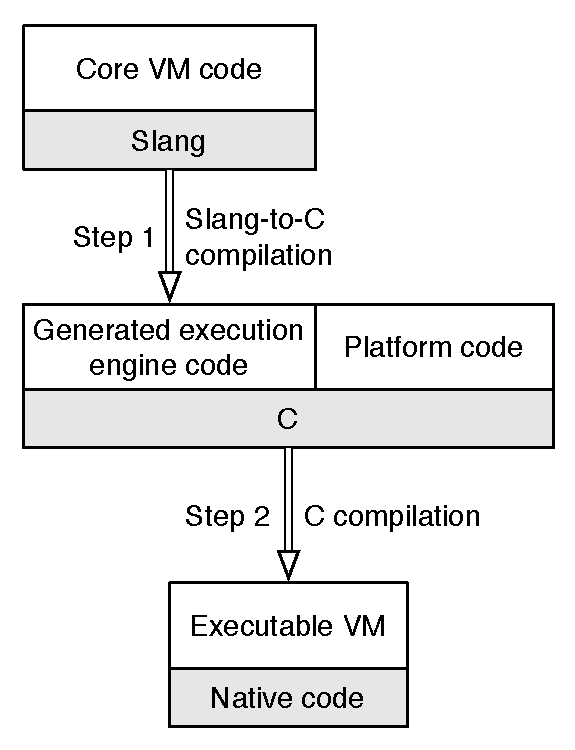
\includegraphics[width=0.6\linewidth]{figures/VMCompilation}
		\caption{Cog VM compilation}
		\label{fig:VMCompilation}
\end{figure}

The executable is generated in two steps as shown on Figure~\ref{fig:VMCompilation}, similarly to the RPython toolchain \cite{RPythonToolchain}. The first step is to generate the two C files representing the whole execution engine written in Slang using the Slang-to-C compiler. During the second step, a C compiler is called to compile the execution engine and the platform-specific code written directly in C to the executable VM.

\cba{We need to introduce here the concept of VM plugin and interpreterproxy indirection/overhead. This is very important since later we just say this is a plugin and we don't redefine it}
\sk{done but someone better check what I wrote :-)}

VM plugins enable the addition of new features to the VM. There are 2 types of plugins: the built-ins and the externals.
\begin{itemize}
\item \emph{External plugins:} Plugins that can be added or removed from the VM without the need to recompile the VM sources.
\item \emph{Internal plugins:} Plugins that cannot be installed without recompiling the VM sources. However, these plugins can reach some parts of the VM internals\footnote{as data structures, routines...} that remains unreachable from an external plugin. These operations are performed via an InterpreterProxy. Although, this solution results in a substential overhead if called often. \cba{Remove from paper InterpreterProxy}
\end{itemize}


\subsection{VM execution}
\label{sec:VMexec}

The Cog VM executes the client's code using an hybrid runtime with an interpreter and a JIT. The interpreter uses a global look-up cache to speed-up virtual calls. On cache hits, it requests the JIT to compile that method and the native code version is used instead. In most case, the JIT is used at the second activation of the method. Closures have similar heuristics.

The VM code, including the interpreter code, is compiled by a C compiler and uses the C stack at runtime. During its execution, the interpreter modifies the execution stack of the client language, which is different from its own code stack as shown on Figure~\ref{fig:TwoStacks}. This means for example that the frame pointer register in the processor refers to a stack frame on the C stack and that a processor push instruction pushes a value on the C stack. When executing the native code generated by JIT, only the client language stack is used. This means for example that the frame pointer register in the processor refers to a stack frame on the client stack and that a processor push instruction pushes a value on the client stack.

\begin{figure}[tbh]
		\centering
		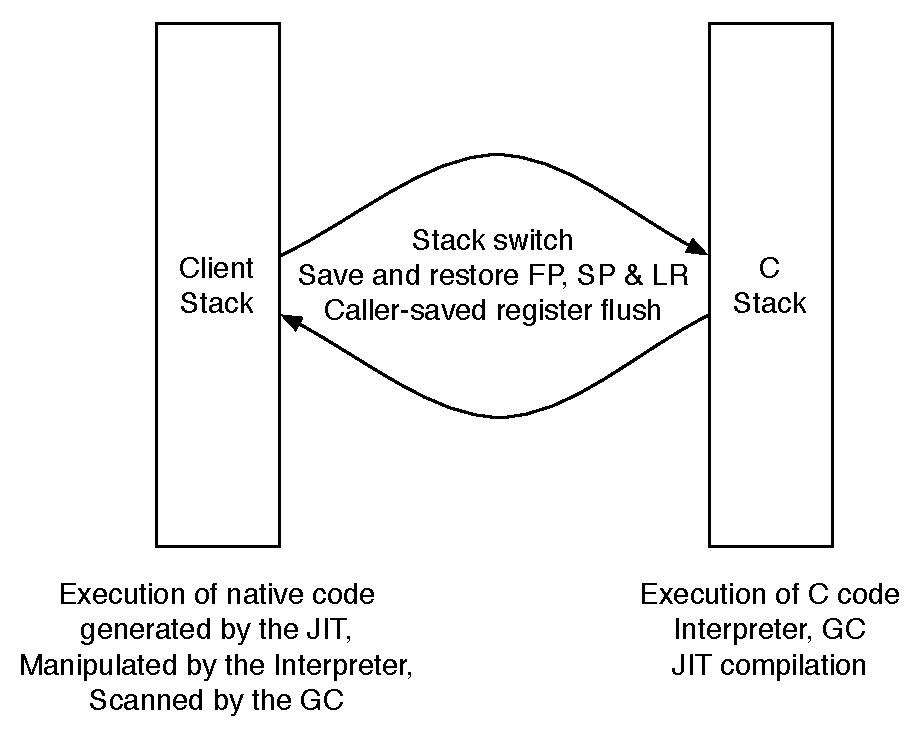
\includegraphics[width=0.99\linewidth]{figures/TwoStacks}
		\caption{Client and C stacks}
		\label{fig:TwoStacks}
\end{figure}

Because of this design, switching the execution between the interpreter and the native code generated by the JIT has a cost. Effectively, the VM needs to switch the frame pointer, the stack pointer and depending on architecture the link register from one stack to the other one. It also needs to save those pointers to be able to resume execution from one stack to the other one. In addition, caller-saved registers on the C conventions or the JIT convention need to be saved since the VM cannot tell ahead what code is going to be used in the other execution model and what registers are required. We estimate the overhead to up to around a dozen of processor instruction, the exact number varies a lot so it is difficult to precise it (the number of register to edit depends on the processor and on the code executed).

Most of the primitives are implemented either in Slang or directly in C. They benefit from the C compiler optimizations to be efficient. When called from the interpreter, activating a primitive is just a C call (the primitive function pointer is cached in the look-up cache next to the method to activate). When called from the native code generated by the JIT, activating a primitive requires to switch the execution from the client stack to the C stack, perform the primitive, and switch back to resume execution. If the primitive takes a significant amount of instructions to execute, for example, the primitive is copying 100kb from one array to another one, the stack switch dance overhead is negligible. If the primitive is very quick to perform, for example, the primitive is adding two integers which do not overflow, the overhead is massive: the execution cost of the addition goes from a few processor instructions to a few dozen instructions.

To solve this performance bottleneck, the Cog VM allows one to redefine primitives in Cog's Register Transfer Language (RTL), an abstract assembly which is compiled to native code through Cog's JIT back-end. Such primitives are then generated to native code at runtime when a method annotated with the primitive is compiled to native code. This allows the primitive to be performed in the client stack with the client calling convention, saving register moves and the stack switch dance. Primitives redefined in such way can be entirely or partially redefined. In the later case, only the common cases are re-implemented on top of the JIT back-end, and an unimplemented case happens at runtime, the generated native code calls the C primitive instead, adding overhead only in uncommon cases.

\subsection{Primitive execution}
\label{sec:primExec}

In the Cog VM, primitives are always associated with compiled methods. A compiled method has information in its header to inform the virtual machine if it has a primitive operation or not. When activating a method with a primitive, the primitive function is executed before the method's bytecode. If the primitive succeeds, the primitive returns a result, as if it were the result of the virtual call. If the primitive fails, it does so without side-effects and execution continues executing the method's bytecode, as if the primitive had not been present.

To fail without side-effects a primitive must validate any parameters and any state fetched from them, before changing execution state by performing its operations. Validation involves any of testing for a specific class, testing for bit vs pointer objects, bounds checks, and recursively applying these tests to substructure of the parameters. For example, the primitive that installs a cursor examines the first parameter to check that it represents a valid cursor object, comprised of two bitmaps, one for the image and one for the shape, plus a point to specify the cursor's hotspot.

The primitives can be associated either with a name, either with an index in the Cog VM. The named primitives can be added and modified without the need to recompile the VM.

\subsection{String comparison primitive}
\label{subsec:primSpec}

\cba{Cette partie je faisais la queue dans la gare en mm temps, a relire}

 The primitive specification is a bit tedious to explain, since as we were trying to improve its performance, we had to change the specifications. In this section we describe first the string implementation, then the original primitive specification and why they were problematic and lastly the new specifications.

\paragraph{String representations.} Strings are represented on top of the Cog VM in two possible forms: ByteStrings and WideStrings. ByteStrings encode each character of the string in a single byte. The encoding usually follows the extended ASCII standard. WideStrings encode each character in 32 bits. The encoding usually follows Unicode specifications. In this paper, we will discuss only the implementation of the string comparison primitive for ByteStrings. WideStrings use an implementation entirely implemented in the client language, and so far, it has not been reported as a performance bottleneck for any program of any users. To sort arrays of strings, strings can be compared. They can be compared in the default order (ASCII or Unicode) or using different orders, for example, the case insensitive order.

\paragraph{Original specification.}  The original primitive took three operands. The two first operands were the two ByteStrings to compare and the third operand was the order table, a ByteArray encoding the order of characters. The default order is the ASCII order, hence each entry corresponds to its index in the byte array (The ByteArray has a size of 256, and accessing the element i, with 0 $\leq$ i $\leq$ 255, answered i). However, in some case, the program may do case insensitive ByteStrings comparison. In this case, the order ByteArray is different, since some entries answer the same value (for example, the entry for the 41 and 61, respectively characters A and a, both answer the same value). To compare two ByteStrings, the primitive conceptually iterates byte by byte over the two objects until it reaches the end of one them, comparing for each byte that the value present in the order ByteArray at the index is greater, equal or smaller than the value computed from the other ByteString. If a difference is met, the value returns based on the result, if not, at the end of the iteration the primitive compares the ByteString sizes and returns. Based on the three parameters, the primitive answered 3, 2, or 1 depending if the first ByteString was greater, equal or smaller than the second one.

\paragraph{Specification issues.} As we were trying to optimize string comparison but specifically string equality, we encountered two main issues:
\begin{itemize}
	\item \emph{Returned value:} Other programming languages implement the primitive to return a negative integer, 0 or a positive integer instead of 1, 2 or 3. It looks like a minor difference, but it is important for performance. With a negative, 0 or positive value, the primitive can just answer the difference between two different characters or the difference in size if all first characters are equal. With 1, 2, or 3, the primitive has to end with multiple branches to know what number to return. In native code, a subtraction is on common architecture quicker to perform than one or multiple branches. In addition, the primitive code is easier to write with the subtraction when writing directly the assembly instructions and we did exactly that when writing the primitive on top of the JIT's back-end.
	\item \emph{Order:} Having the order as the third operands is convenient in some cases (case insensitive comparison), but is just overhead in the common case (checking for string equality).
\end{itemize}

\paragraph{Final specification.} The final specification we productized last month takes two or three parameters. The third parameter, the order, is optional. If the third parameter is absent, the VM assumes the byte ordering (ASCII order) is the order to compare against. Therefore, the VM does not need to go through the indirection order array in the common case. The primitive answers a negative integer, zero, or a positive integer as the first parameter is less than, equal to, or greater than the second parameter.

In the paper we will focus on the comparison of two strings with the default ASCII ordering and measure the performance only of this case. The goal of this work was to improve the performance of common string operations, typically string equality which internally use the primitive, and the cases where the order is non ASCII are uncommon.

\section{Different primitive implementations}
\label{sec:implem}

 This section first describes the different ways of implementing a primitive. We then explain how each of these versions are executed by the VM and the pros and cons of each and every.

 \subsection{Different implementations and executions}

\paragraph{Baseline: pure Smalltalk.}
To evaluate the primitive performance, we use as baseline an implementation in pure Smalltalk. There are multiple ways of writing the comparison of two strings in Smalltalk, following Smalltalk coding conventions, a standard developer would likely use high-level constructs which apply a closure on each element of the strings. We did not use high-level construct and chose to implement the Smalltalk version the most optimized way Smalltalk allows, \emph{i.e.,} we used the contructs to:do: and ifFalse:, which are both recognized by the Smalltalk to bytecode compiler and compiled respectively to loops and branches at the bytecode level. The implementation follows the new specification, hence two methods are available, baselineCompareWith: and baselineCompareWith:order:. Since the focus is only on ASCII ordered comparison, we show the code only of baselineCompareWith:.

\begin{code}
baselineCompareWith: aString
	| c1 c2 length1 length2 |
	length1 := self size.
	length2 := aString size.
	1 to: (length1 min: length2) do: [ :i |
		(c1 := self basicAt: i) = (c2 := aString basicAt: i) ifFalse: [ ^ c1 - c2 ] ].
	^ length1 - length2
\end{code}

\paragraph{Existing: Smart Syntax Plugin.}

The Smart Syntax Plugin is one of the version existing until we started this work. The idea behind Smart Syntax was the following: the programmer can write code in Smalltalk using exclusively constructs that are recognized by the Smart Syntax compiler and that can be directly compiled to C (computing the size of a byte array, accessing its fields and doing integer arithmetic for example). With the addition of type annotations in the form of pragmas \cite{Duca16a} \footnote{Pragma are a form of method annotation.}, the Smart Syntax plugin was able to generate C code from the Smalltalk code. With this approach, the programmer has to write the optional primitive code a single time in Smalltalk. This code is used both as the fall-back code if the VM does not implement the primitive and at Slang to C compilation time to generate a C plugin from the code and the type annotations. This primitive follows the old specification, the full code is available in Appendix \ref{SmartSyntaxAppendix}.

\paragraph{Existing: Slang Plugin.}

The Slang plugin is a recent complete rewrite of the Smart Syntax plugin. The main difference is that the Smalltalk version is used only as fall-back code, while at Slang to C compilation time the VM uses code written in Slang to generate the C code. One of the side-effect is that the plugin's code is now part of the VM code base and not the client code bases, which is convenient for maintenance since the Cog VM has multiple client languages. However, the implementor now needs to maintain and evolve two version of the primitive, the fall-back code in Smalltalk and the code in Slang. This primitive follows the old specification, the full code is available in Appendix \ref{PluginAppendix}.

\paragraph{Pure Slang.}

The Slang implementation is written inside the interpreter and has access to all interpreter APIs. Since the same primitive index is used for the primitive with 2 or 3 arguments, the primitive needs to deal with both cases in a way that the common case is efficient. The primitive is now part of the core of the VM, it cannot be easily added or removed as plugin primitives, but it is simpler to read and write. This primitive follows the new specification, the full code is available in Appendix \ref{SlangAppendix}.

\paragraph{Pure Slang with JIT support.}

In addition to the previous implementation, we've re-implemented here the primitive on top of Cog's JIT back-end. The primitive is written in Cog's RTL, an abstract assembly which instructions compile almost one-to-one to native instructions. This primitive requires a more important amount of work to be written: the number of line of code is greater, the implementor has to be careful to generate efficient machine code (there is no C compiler to optimize the code) and debugging such code requires the use of a processor simulator. Since only performance critical implementations matter in this context, we've re-implemented only the case where there is 2 parameters. For the three parameter primitive, the VM falls-back to the Slang version. This primitive follows the new specification, the full code is available in Appendix \ref{RTLAppendix}.

\subsection{Comparison}
\label{sec:implem_cmp}

\begin{table*} [bth]
\centering
\begin{tabular}{c|cccc|ccc}
   &  \multicolumn{4}{c|}{Software maintenance \& evolution} & \multicolumn{3}{c}{Primitive execution time}\\
  \hline
    & Recompilation & Familiar to & Lignes & Number of & Stack switch & Optimization & Code generation \\
    & required & developers & of code & implementations & overhead & potential & control \\
  \hline
  Baseline    & No & All  & 10  & 0 & No & - & - \\
   \hline
  SmartSyntax & Plugin & VM & 20  & 3+ & Yes  & Limited & Low \\
   \hline
  SlangPlugin & Plugin & VM & 35  & 1  & Yes & Limited & Low \\
   \hline
  PureSlang   & Yes  & VM & 45  & 1  & Yes & High & Low \\
   \hline
  Slang+JIT   & Yes  & VM-JIT & 85  & 2  & No & High & High \\
  \hline
\end{tabular}
\caption{Comparison between implementations\vspace{-0.5cm}}
\label{tab:cmp_implem}
\end{table*}

 In this section we compare the five different implementations according to the following criteria:
 \begin{itemize}
 	\item \emph{Recompilation required:} Changing the implementation requires only Smalltalk bytecode recompilation (No), requires to recompile a plugin to a dynamic library if compiled as external or the recompilation of the full VM if compiled as internal (Plugin) or requires to recompile the full VM (Yes).
	\item \emph{Implementation language familiar to developers:} Smalltalk application developers are considered to be familiar with Smalltalk only, while Cog VM developers are considered being familiar with Smalltalk, Slang, C and Assembly code. Only Cog's JIT implementors are familiar with its RTL, which is a subset of the VM developers.  We use \emph{All} if all communities are familiar with the language, \emph{VM} if all VM developers are and \emph{VM-JIT} if only a subset of VM developers are.
	\item \emph{Readability:} To evaluate the readability of the approach, we use one of the most used metric, the number of lines of code.
	\item \emph{Number of implementations to maintain:} In each case, the client language has to implement a fall-back code in Smalltalk to execute if the primitive fails. This code is maintain by the client language implementors, and not by the VM implementors. Hence we do not count the fall-back code in the number of implementation to maintain, nor the pure Smalltalk implementation. However, as a VM implementor, we need to maintain what generates the C code of the VM, hence, in the case of Smart Syntax, we need to maintain a different method in each client language. We also count all the Slang implementations as well as the ones on Cog's RTL.
	\item \emph{Stack switch overhead:} Yes if activating the primitive from the native code generated by the JIT requires to switch between the C and the client stack, inducing execution time overhead.
	\item \emph{Optimization potential:} \cba{need to mention that this is for large strings}
	C cross-file inlining is not performed by default for internal plugins. External plugins don't have access to the whole VM API and have to go through InterpreterProxy to do so, leading to an overhead. \cba{InterpreterProxy not defined before}
	\item \emph{Control over the generated code:} The implementations written in Slang are compiled by the C compilers into native code. The generated code can therefore differ according the compilers and the optimizations they performed. On the contrary, the JIT will always generate the same native code.
\end{itemize}

One or another implementation could be preferred depending on the intended aim: the main trade-off will be found between the engineering time and the performance. Table \ref{tab:cmp_implem} summarizes the main pros and cons related to each implementation: the engineering time may tend to increase when more low-level languages are used, such as Cog's RTL for instance.
Also, a VM recompilation affects the overall complexity of the development process, but the resulting code might be faster to run. Likewise, the use of plugins may bring modularity, but as you will see in Section \ref{sec:eval}, the performance, although better than baseline version, could still be improved.

\cba{In this section somewhere we need to say that criteria are split in maintenance and performance, the evaluation in next section is on last 3 criteria: Stack switch overhead, Optimization potential and control over the generated code.}

\section{Evaluation}
\label{sec:eval}

The SlangPlugin, PureSlang and Slang+JIT implementations of this string comparison primitive have been recently implemented in the Cog VM. In this section, we will compare the performances of these primitives against the other existing implementations performances. We have measures their respective execution times for different string sizes.

\subsection{Set-up}

\paragraph{GCC-Linux.}The GCC-Linux evaluation was performed on an Asus Zenbook with Ubuntu 16.04 LTS, a 2.2 Ghz processor Intel Core 5, 8 Gb 1600MHz DDR3 of RAM. The Linux VM was compiled using GCC version 5.4.0.

\paragraph{LLVM-Mac.}The LLVM-Mac evaluation was performed on a MacBook pro with Mac OS 10.11.6, a 2.9 Ghz processor Intel Core 5, 8 Gb 1867MHz DDR3 of RAM. The Mac VM was compiled using Apple LLVM version 8.0.0 (clang-800.0.38).

\paragraph{Processor.}The following evaluation was performed on 32 bits Intel VMs (x86).

\subsection{Methodology}

We assessed the execution time of the different implementations by running the following benchmark:

\begin{code}
#(0 1 5 100 1000) collect: [ :size |
	| iterations time overhead |
	collection := ByteString new: size.
	collection2 := ByteString new: size.
	size < 100 
		ifTrue: [iterations := (100000000 // (size*10 max: 1) sqrt) floor.]
		ifFalse: [iterations := (10000000 // size sqrt) floor.].
	overhead := [ 1 to: iterations do: [ :i | ] ] timeToRun.
	time := [ 1 to: iterations do: [ :i |
		collection compareWithSlang: collection2 ] ] timeToRun.
	stream nextPutAll: ((time - overhead) asString)].
\end{code}\\

Each benchmark was measured 30 times.

%%%
% Legend definition (so I can change it once for all)
%%%

\def\legBase{Baseline}
\def\legSmartSyntaxPlug{Smart syntax}
\def\legSlangPlug{Plugin}
\def\legSlang{Pure slang}
\def\legRTL{Slang+JIT}
\def\plotHeight{6.4cm}

%%%
% End Legend
%%%

\begin{figure*}[htb!]
  \centering
    \begin{subfigure}[b]{\textwidth}
    \begin{subfigure}[b]{.19\textwidth}
    \subcaption*{Size 0}
    \begin{tikzpicture}
      \begin{axis}
      [
        height=\plotHeight,
        x=0.5cm,
        xtick={1,...,5},
        xticklabel style={rotate=90},
        bar width=0.3cm,
        enlarge x limits={abs=0.45cm},
        xticklabels={\legBase, \legSmartSyntaxPlug, \legSlangPlug, \legSlang, \legRTL},
        font={\footnotesize},
	ybar=10pt,
	ymin=0
        ]
\addplot[
    fill=black!25,
    draw=black,
    fill,
    point meta=y,
    every node near coord/.style={inner ysep=5pt},
    error bars/.cd,
        y dir=both,
        y explicit
]
table [y error=error] {
x   y           error
1   1           0
2   0.3411212   0.0006746299
3   0.3375418   0.001577878
4   1.077762   0.005363974
5   2.490423    0.004304882
};
      \end{axis}
    \end{tikzpicture}
    \end{subfigure}
     \begin{subfigure}[b]{.19\textwidth}
    \subcaption*{Size 1}
    \begin{tikzpicture}
      \begin{axis}
      [
        height=\plotHeight,
        x=0.5cm,
        xtick={1,...,5},
        xticklabel style={rotate=90},
        bar width=0.3cm,
        enlarge x limits={abs=0.45cm},
        xticklabels={\legBase, \legSmartSyntaxPlug, \legSlangPlug, \legSlang, \legRTL},
        font={\footnotesize},
	ybar=10pt,
	ymin=0
        ]
\addplot[
    fill=black!25,
    %draw=none,
    %fill,
    draw=black,
    fill,
    point meta=y,
    every node near coord/.style={inner ysep=5pt},
    error bars/.cd,
        y dir=both,
        y explicit
]
table [y error=error] {
x   y           error
1   1           0
2   0.6013716   0.0023206431
3   0.5653467   0.007829291
4   1.816869    0.019114984
5   3.537800    0.012357500
};
      \end{axis}
    \end{tikzpicture}
    \end{subfigure}
    \begin{subfigure}[b]{.19\textwidth}
    \subcaption*{Size 5}
    \begin{tikzpicture}
      \begin{axis}
      [
        height=\plotHeight,
        x=0.5cm,
        xtick={1,...,5},
        xticklabel style={rotate=90},
        bar width=0.3cm,
        enlarge x limits={abs=0.45cm},
        xticklabels={\legBase, \legSmartSyntaxPlug, \legSlangPlug, \legSlang, \legRTL},
        font={\footnotesize},
	ybar=10pt,
	ymin=0
        ]
\addplot[
    fill=black!25,
    draw=black,
    point meta=y,
    every node near coord/.style={inner ysep=5pt},
    error bars/.cd,
        y dir=both,
        y explicit
]
table [y error=error] {
x   y           error
1   1           0
2   1.3891212   0.0029489731
3   1.3149840   0.020471694
4   3.818961   0.054523074
5   6.740474    0.010805042
};
      \end{axis}
    \end{tikzpicture}
    \end{subfigure}
    \begin{subfigure}[b]{.19\textwidth}
    \subcaption*{\hspace{0.4cm}Size 100}
 \begin{tikzpicture}
      \begin{axis}
      [
        height=\plotHeight,
        x=0.5cm,
        xtick={1,...,5},
        xticklabel style={rotate=90},
        bar width=0.3cm,
        enlarge x limits={abs=0.45cm},
        xticklabels={\legBase, \legSmartSyntaxPlug, \legSlangPlug, \legSlang, \legRTL},
        font={\footnotesize},
	ybar=10pt,
	ymin=0
        ]
\addplot[
    fill=black!25,
    draw=black,
    point meta=y,
    every node near coord/.style={inner ysep=5pt},
    error bars/.cd,
        y dir=both,
        y explicit
]
table [y error=error] {
x   y           error
1   1           0
2   8.6795487   0.0586762222
3   8.9585208   0.116958804
4   15.809515   0.300447885
5   16.752667    0.106255682
};
      \end{axis}
    \end{tikzpicture}
    \end{subfigure}
    \begin{subfigure}[b]{.19\textwidth}
    \subcaption*{\hspace{0.5cm}Size 1000}
     \begin{tikzpicture}
      \begin{axis}
      [
        height=\plotHeight,
        x=0.5cm,
        xtick={1,...,5},
        xticklabel style={rotate=90},
        bar width=0.3cm,
        enlarge x limits={abs=0.45cm},
        xticklabels={\legBase, \legSmartSyntaxPlug, \legSlangPlug, \legSlang, \legRTL},
        font={\footnotesize},
	ybar=10pt,
	ymin = 0
        ]
\addplot[
    fill=black!25,
    draw=black,
    point meta=y,
    every node near coord/.style={inner ysep=5pt},
    error bars/.cd,
        y dir=both,
        y explicit
]
table [y error=error] {
x   y           error
1   1           0
2   13.6051267   0.0589164968
3   14.7789145   0.147140189
4   24.417751   0.186326223
5   24.480071    0.095038374
};
      \end{axis}
    \end{tikzpicture}
   \end{subfigure}
  % \caption{GCC-Linux results}
   % \label{fig:gcc}
   \subcaption*{\textbf{GCC-Linux}\vspace{0.25cm}}
   \label{fig:gcc}
   \end{subfigure}
 \begin{subfigure}[b]{\textwidth}
    \begin{subfigure}[b]{.19\textwidth}

    \begin{tikzpicture}
      \begin{axis}
      [
        height=\plotHeight,
        x=0.5cm,
        xtick={1,...,5},
        xticklabel style={rotate=90},
        bar width=0.3cm,
        enlarge x limits={abs=0.45cm},
        xticklabels={\legBase, \legSmartSyntaxPlug, \legSlangPlug, \legSlang, \legRTL},
        font={\footnotesize},
	ybar=10pt,
	ymin=0,
	]
\addplot[
    fill=black!25,
    draw=black,
    point meta=y,
    every node near coord/.style={inner ysep=5pt},
    error bars/.cd,
        y dir=both,
        y explicit
]
table [y error=error] {
x   y           error
1   1           0
2   0.3147064   0.002288488
3   0.3035965   0.001786185
4   0.8545431   0.006132950
5   2.250732    0.04133638
};
      \end{axis}
    \end{tikzpicture}

    \end{subfigure}
     \begin{subfigure}[b]{.19\textwidth}

    \begin{tikzpicture}
      \begin{axis}
      [
        height=\plotHeight,
        x=0.5cm,
        xtick={1,...,5},
        xticklabel style={rotate=90},
        bar width=0.3cm,
        enlarge x limits={abs=0.45cm},
        xticklabels={\legBase, \legSmartSyntaxPlug, \legSlangPlug, \legSlang, \legRTL},
        font={\footnotesize},
	ybar=10pt,
	ymin=0
        ]
\addplot[
    fill=black!25,
    draw=black,
    point meta=y,
    every node near coord/.style={inner ysep=5pt},
    error bars/.cd,
        y dir=both,
        y explicit
]
table [y error=error] {
x   y           error
1   1           0
2   0.5605682   0.002198180
3   0.5566675   0.001023225
4   1.5605275   0.006372279
5   3.754532    0.01109086
};
      \end{axis}
    \end{tikzpicture}

    \end{subfigure}
    \begin{subfigure}[b]{.19\textwidth}

    \begin{tikzpicture}
      \begin{axis}
      [
        height=\plotHeight,
        x=0.5cm,
        xtick={1,...,5},
        xticklabel style={rotate=90},
        bar width=0.3cm,
        enlarge x limits={abs=0.45cm},
        xticklabels={\legBase, \legSmartSyntaxPlug, \legSlangPlug, \legSlang, \legRTL},
        font={\footnotesize},
	ybar=10pt,
	ymin=0
        ]
\addplot[
    fill=black!25,
    draw=black,
    point meta=y,
    every node near coord/.style={inner ysep=5pt},
    error bars/.cd,
        y dir=both,
        y explicit
]
table [y error=error] {
x   y           error
1   1           0
2   1.2505193   0.004611354
3   1.2295801   0.001810171
4   2.8205415   0.008035024
5   7.089806    0.01403785
};
      \end{axis}
    \end{tikzpicture}
    \end{subfigure}
    \begin{subfigure}[b]{.19\textwidth}
 \begin{tikzpicture}
      \begin{axis}
      [
        height=\plotHeight,
        x=0.5cm,
        xtick={1,...,5},
        xticklabel style={rotate=90},
        bar width=0.3cm,
        enlarge x limits={abs=0.45cm},
        xticklabels={\legBase, \legSmartSyntaxPlug, \legSlangPlug, \legSlang, \legRTL},
        font={\footnotesize},
	ybar=10pt,
	ymin=0
        ]
\addplot[
    fill=black!25,
    draw=black,
    point meta=y,
    every node near coord/.style={inner ysep=5pt},
    error bars/.cd,
        y dir=both,
        y explicit
]
table [y error=error] {
x   y           error
1   1           0
2   6.6951738   0.062391122
3   6.6032572   0.024774416
4   10.3029394  0.061481532
5   17.979611   0.10127936
};
      \end{axis}
    \end{tikzpicture}
    \end{subfigure}
    \begin{subfigure}[b]{.19\textwidth}

    \begin{tikzpicture}
      \begin{axis}
      [
        height=\plotHeight,
        x=0.5cm,
        xtick={1,...,5},
        xticklabel style={rotate=90},
        bar width=0.3cm,
        enlarge x limits={abs=0.45cm},
        xticklabels={\legBase, \legSmartSyntaxPlug, \legSlangPlug, \legSlang, \legRTL},
        font={\footnotesize},
	ybar=10pt,
	ymin=0
        ]
\addplot[
    fill=black!25,
    draw=black,
    point meta=y,
    every node near coord/.style={inner ysep=5pt},
    error bars/.cd,
        y dir=both,
        y explicit
]
table [y error=error] {
x   y           error
1   1           0
2   9.4064534   0.036698187
3   9.2138415   0.013982843
4   13.4384830  0.040202717
5   26.404792   0.09298324
};
      \end{axis}
    \end{tikzpicture}

   \end{subfigure}
   \subcaption*{\textbf{LLVM-Mac}\vspace{-0.2cm}} %change vspace based on fig position
    \end{subfigure}
   \caption{String comparison benchmarks for strings of different sizes on different architectures}
   \label{fig:bench}
\end{figure*}
\begin{table*}
\centering
\begin{tabular}{|c|c|c|c|c|c|c|}
  \hline
    & & 0 & 1 & 5 & 100 & 1000 \\
   \hline
  \multirow{2}{*}{SmartSyntax} &GCC & 0.3411 +- 0.0007 & 0.6014 +- 0.0023 & 1.3891 +- 0.0023 &  8.6796 +- 0.0587 & 13.6051 +- 0.0589\\
 							   &LLVM & 0.3147 +- 0.0023 & 0.5606 +- 0.0022 & 1.2505 +- 0.0046 & 10.3029 +- 0.0624 & 9.4065 +- 0.0367\\
   \hline
  \multirow{2}{*}{SlangPlugin} &GCC& 0.3375 +- 0.0016 & 0.5654 +- 0.0078 & 1.3150 +- 0.0205 & 8.9585 +- 0.1170  & 14.7789 +- 0.1471 \\
  							   &LLVM& 0.3036 +- 0.0018 & 0.5567 +- 0.0010 & 1.2296 +- 0.0018 & 6.6033 +- 0.0248  & 9.2138 +- 0.0140 \\
   \hline
  \multirow{2}{*}{PureSlang} &GCC& 1.0778 +- 0.0054 & 1.8169 +- 0.0191 & 3.8190 +- 0.0545 & 15.8095 +- 0.3005 & 24.4178 +- 0.1863\\
 							 &LLVM& 0.8545 +- 0.0061 & 1.5605 +- 0.0064 & 2.8205 +- 0.0080 & 10.3029 +- 0.0615  & 13.4385 +- 0.0402 \\
   \hline
  \multirow{2}{*}{Slang+JIT} &GCC& 2.4904 +- 0.0043 & 3.5378 +- 0.0124  & 6.7405 +- 0.0108 & 16.7527 +- 0.1063 & 24.4801 +- 0.0950\\
 							&LLVM & 2.2507 +- 0.0413 & 3.7545 +- 0.0111 & 7.0898 +- 0.0140 & 17.9796 +- 0.1013  & 26.4048 +- 0.0930 \\
  \hline
\end{tabular} 
\vspace{0.2cm}
\caption{Benchmark results with standard errors. Average relative speed-up regarding baseline}
\label{tab:detail_bench}
\end{table*}

\begin{figure*}[b!]
		\centering
		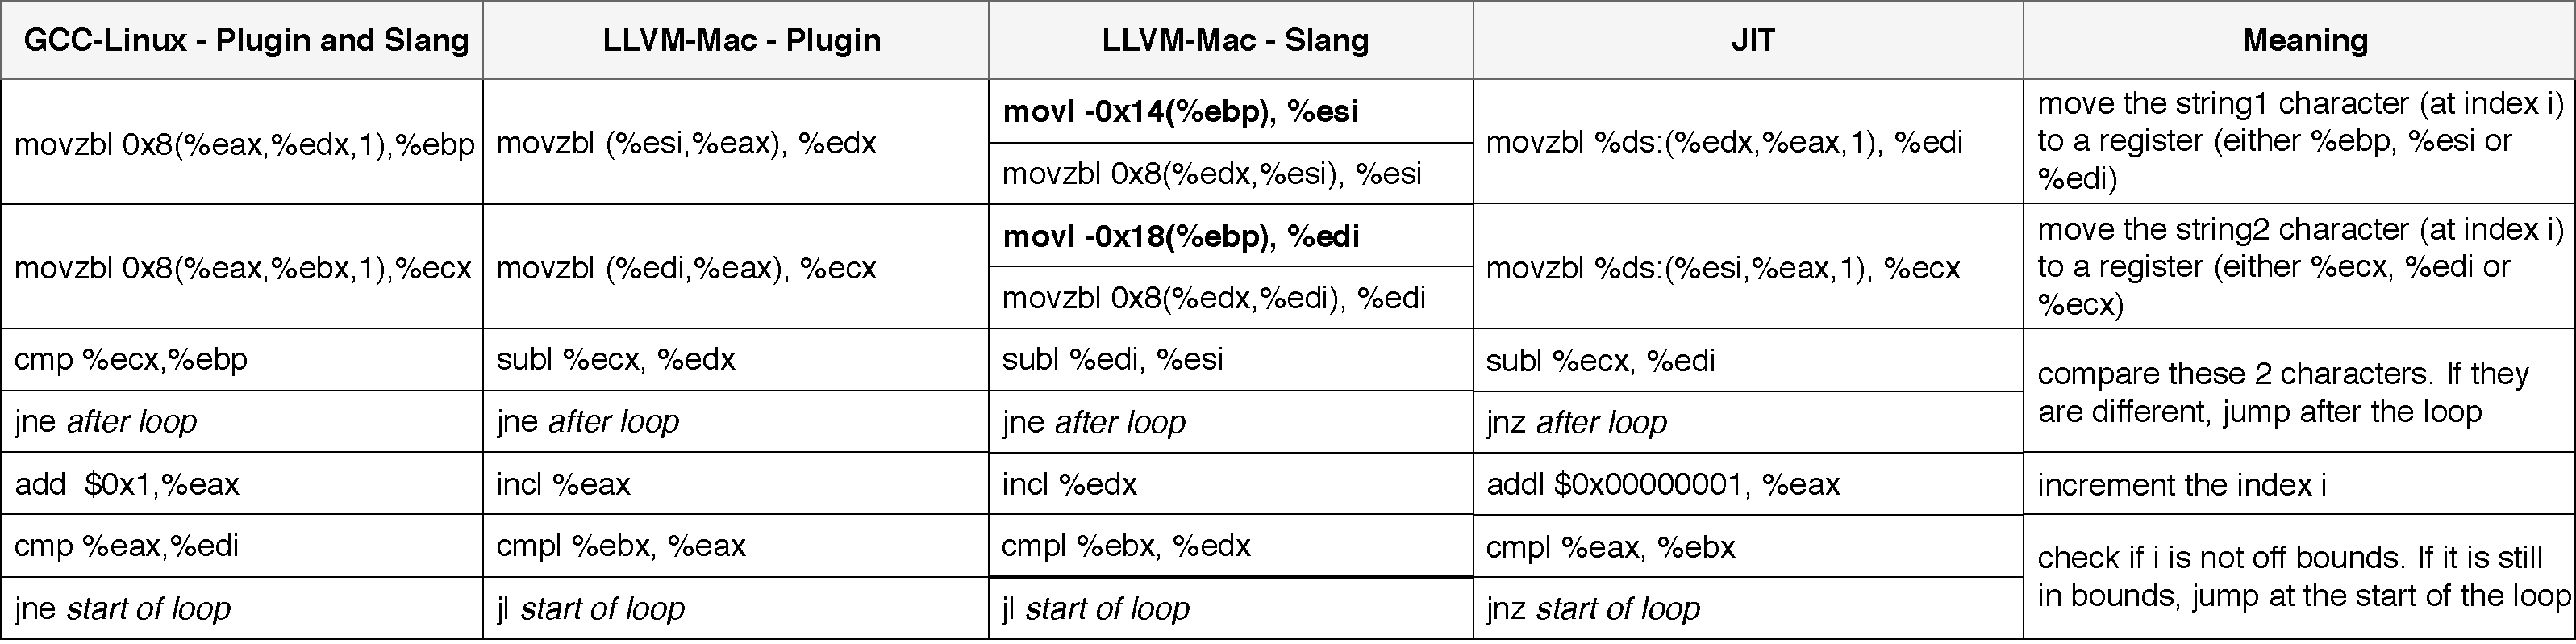
\includegraphics[width=1\linewidth]{figures/asm_cmp.pdf}
		\caption{GCC and LLVM: different optimizations on the comparison loop}
		\label{fig:Asm}
\end{figure*}

In each benchmark, we run a string comparison in a loop and measure the total execution time.
The number of iterations of the loop depends on the string size: the comparison is repeated between 1414 and 10000 times for a short string (5 characters or less), and between 100 and 316 times for a long string (100 characters or more). This addresses the warm-up of the JIT \cba{??? This needs to be explained differently. We get into jitted code after a small number of loop iteration (I think 20 currently) or second call. The JIT overhead is negligible here for 1 second because we could not see any time spent in the JIT in the profiler + ref to your paper, i.e. less than 0.5ms in the JIT} \cite{CogProfiler} and allows the benchmarks to run at least 1 second in the slower implementations \cba{Ok, 1 second to avoid processor / OS noises, not just for fun}.
The loop overhead is measured and removed from the measurements. 

The two compared strings are equal as it corresponds to the worst scenario for most of our benched implementations. There is one less branch in the two plugin implementations in this case.

\subsection{Micro-benchmarks}

%\cba{Je pense string de taille 0-1 c'est cool pour montrer que le code C va moins vite que pur smalltalk dans ce cas (si c'est vraiment le cas)}
We performed the benchmarks upon five different string sizes: 0, 1, 5, 100 and 1000 characters, using two different compilers: GCC on one hand and LLVM on the other hand. Figure \ref{fig:bench} show the results in terms of relative speed-up towards the baseline implementation, respectively for GCC and LLVM.


We can draw the following patterns from these results:
\begin{itemize}
\item The execution time of the SmartSyntax and Plugin implementations is either very close or greater than the baseline's for the small strings.
\item The Slang+JIT implementation is more efficient than the baseline in every case. Nevertheless,the performance gap between this version and the PureSlang one tends to decrease as the string size increases. 
\item The compiler used (either GCC or LLVM) does not lead to significant differences in terms of performance, except for the 100+-characters strings. 
\end{itemize}

We can explain these results based on the last 3 criteria detailed in Section \ref{sec:implem_cmp}:

\paragraph{Stack switch overhead.}
As mentionned in Section \ref{sec:VMexec}, all implementations written in Slang come with an overhead due to the switch between the C and Smalltalk stacks. This overhead is clearly visible in the bench results in Figure \ref{fig:bench} for small strings (size 1 or less): the SmartSyntax and Plugin implementations are around 30 to 60\% slower than the baseline's, and the PureSlang performances are close to the baseline's.
As the string size goes larger, the overhead is less significant because it is **absorbed** by other performance gains.
Regarding this criteria, the Slang+JIT version is always the fastest: it is not really impacted by the switch overhead, because the Slang part is used for a very short time.

\paragraph{Optimization potential on large strings comparison.}
The plugins come with an overhead \sk{not an overhead when it comes to inlining. Just not optimized. need rephrasing} due to the cross-file inlining and the passage through an InterpreterProxy, like said in Section \ref{sec:implem_cmp}. This is one of the factor explaining the performance gap between these versions and the Slang and Slang+JIT ones.
When it comes to comparing large strings (100 characters and more), the execution time is mainly spent in the comparison loop (Figure \ref{fig:Asm}). However, the switch overhead is still noticeable in the PureSlang implementation when strings of 100 characters are compared: PureSlang is 15.8 times faster while Slang+JIT is 16.8 times faster. This is not the case anymore on 1000-characters strings.
This last observation only applies to the GCC results: the code generated by the LLVM compiler induces a longer execution time, as explained in the next paragraph. 

One could notice a rather striking performance difference between the 2 compilers: when compiling with GCC, the performances between the PureSlang and Slang+JIT implementations are really close for long strings (100 characters and longer), with respectively 24,42 and 24,48 relative speed-up factors for a 1000-characters string. Yet they greatly differ when LLVM is used, with respectively 13,44 and 26,40 relative speed-up factors.

This difference is mainly due to the optimizations performed by both the compilers: as depicted in Figure \ref{fig:Asm}, GCC generates instructions that are very close to the ones generated by the JIT, hence the similar speed-up factors. On the contrary, LLVM generates more instructions: it especially fails at preserving the registries holding the strings (edi and esi), leading to 2 extra instructions (bolded in the figure) that will load the strings at each iteration.

\todo{add conclusion}



%We can draw the following patterns from these results:
%\begin{itemize}
%\item The execution time of the SmartSyntax and Plugin implementations is either very close or greater than the baseline's for the small strings. This can be explained by the high cost of the switching between the C and Smalltalk stacks, as mentionned in Section \ref{sec:VMexec}.
%\item The Slang+JIT implementation is more efficient in every case. Nevertheless,
%the performance gap between this implementation and the PureSlang one tends to decrease as the string size increase. The comparison loop (\ref{fig:Asm}) proves to be more and more time-consuming because of the higher number of iterations.
%\end{itemize}
%
%\todo{Following comments are the most important for paper}
%
%\cba{we had 3 criterias:
%- 1 C ST stack switch overhead. 
%- 2 optimization potential, that we may change to large string cmp perf
%- 3 control over generated code
%We need to explain the results based on each criteria, ideally in 3 paragraphs entitled with the 3 criteria.
%The 2 paragraph below explain only point 3 and lacks a conclusion sentence "blabla we have control and if C compiler is not good such as uncommon back-end or x86 which is still quite common in this case..."
%}
%\cba{This is the kind of missing things: C ST stack switch overhead: small string, overhead stack switch high, baseline and JIT version fastest. 
%Large string perf: Large string, loop is where the time is spent, slang and JIT fastest.
%We need size 1000 so that the stack switch overhead cannot be seen anymore on gcc (size 100 we still C it)}
%
%\cba{Maybe small discussion on relevance
%Size 0 is only '' = '', not really interesting in real app, but show well the stack switch overhead.
%Example use cases are comparing tokens in parsers (Size ~4-10 [self, super, thisContext, this, etc.])
%Other example are long urls, hundreds of characters, which are represented with large string comp bench
%or something like that.}
%
%However, one could notice a rather striking performance difference between the 2 compilers: when compiling with GCC, we notive in Figure \ref{fig:bench} that the performances between the PureSlang and Slang+JIT implementations are really close for long strings (100 characters and longer), with respectively 24,42 and 24,48 relative speed-up factors for a 1000-characters string. Yet they greatly differ when LLVM is used, with respectively 13,44 and 26,40 relative speed-up factors.
%
%This difference is mainly due to the optimizations performed by both the compilers: as depicted in Figure \ref{fig:Asm} GCC generates instructions that are very close to the ones generated by the JIT, hence the similar speed-up factors. On the contrary, LLVM generates more instructions: it especially fails at perserving the registries holding the strings (edi and esi), leading to 2 extra instructions (bolded in the figure) that will load the strings at each iteration.

\section{Discussion and related work}

\cba{Maybe talk in those cases the number of representation of the primitives, this is a bit disconnected with the rest of the paper I feel}

We identified two directly related works. In some languages (Strongtalk, Self, RSqueak), the implementors tried to decrease the overall number of optional primitives by improving the client language performance, reducing the need for such primitives \cite{Strongtalk, ursPHD, NoPrimTracing}. In addition, in the V8 project  \cite{V8}, the interpreter was entirely built on top of the V8 JIT's back-end using a specific DSL similar to Cog's RTL.

\subsection{Decreasing the number of primitives}

The philosophy of Self and Strongtalk, both high performance VMs, were to improve the performance of the client language with a mature optimizing JIT featuring advanced optimizations such as speculative optimizations \cite{Strongtalk, ursPHD}. In this context, the need of primitive is reduced, since the performance gain from using a primitive over the client language is low or inexistant. More recently, Felgentreff \emph{et al.} \cite{NoPrimTracing} analysed the performance difference between primitives implemented in C, RPython, and Smalltalk. They showed that with the RPython toolchain framework, the performance difference between all three implementation was not that big, hence they could choose to implement some optional primitives in the client language over C or RPython without performance drop to reduce the number of primitives to maintain.

These approaches have the advantage of decreasing the primitive maintenance cost since fewer primitives have to be maintained. The performance problem is however partially solved: only the peak performance is similar with and without the primitives. Since those system rely on JITs, start-up performance is worse than peak performance, increasing the performance difference at start-up between the client code and the primitive. In addition, the performance can be  unreliable with optimizing JITs. The implementors of Morphic \cite{MorphicSelf} on top of the Self VM were complaining that changing a single line of code could lead to important performance drop and they would not understand why. Those performance drops were due to the optimizing JIT taking different optimization decisions. This problem was so significant that recently the V8 team \cite{V8} rewrote their primitives written in Javascript (named built-ins in their project) in a DSL compiled ahead of time through their JIT back-end to improve the performance of the primitives and therefore decrease the performance drop between baseline and peak performance. Aside from the start-up performance and the performance unreliability problems described, these approaches also require a mature optimizing JIT, hard to implement and maintain.

\subsection{No stack switch overhead}

To avoid paying the stack switch cost between the client Stack and the C stack, the V8 team recently wrote an interpreter Ignition in a DSL compiled ahead of time through their JIT back-end to native code. With their primtives and their interpreter written in the DSL, the V8 runtime rarely needs to switch between the client and the C stack (no need to switch to interpret code, no need to switch for primitives). In this context, the stack switch overhead is not a problem anymore.

In our context, implementing a similar approach would require us to compile Slang to native code through our JIT compiler back-end or to rewrite the interpreter on top of Cog JIT's RTL. Slang has some abstractions over native code, similarly to C. Compiling Slang ahead of time to native code efficiently requires us to re-implement optimizations implemented in C compilers and we don't want that complexity or to lower the abstractions level of Slang to express native code optimizations, which would increase the complexity of Slang, which we don't want either. Rewriting the interpreter on top of Cog JIT's RTL is possible but requires a significant amount of work.

\section{Future work and conclusion}

In this section we discuss two future work directions and conclude.

\paragraph{Future work: back-end specific.}

All the primitive we compare are written in a processor independent way, due to the C compiler abstraction for the Slang versions, the abstract assembly abstraction for Cog's RTL version or the VM abstraction for the baseline implementation in Smalltalk. We could rewrite the primitive differently for each back-end currently supported (x86, x64, MIPSEL, ARMv6) and yet to support (ARMv8, ...). It could be relevant in some cases performance-wise, for example, on intel processors, the JVM implements string comparison using the SSE4.2 string comparison instructions when available \cite{JVMSSE4StringComp}. We did not go in this direction because the maintenance cost in this case is definitely too high since we would have to maintain a different implementation per back-end  (already 4 implementations today).

\paragraph{Future work: adaptive optimizer integration.}

For the past few years, an experimental adaptive optimizer (a JIT featuring advanced optimizations such as speculative inlining) has been developed on top of the Cog VM \cite{SistaFastStartUp}. The optimizer has specific rules to be able to inline primitive operations without performance loss. We need to carefully measure, in different benchmarks, the performance of the inlined string comparison primitive. We also need to discuss the maintenance cost, for example, do we need a new representation of the primitive for the optimizing JIT to inline it? The micro-benchmarks used in the paper were relevant to show the client stack to C stack switch overhead as well as baseline performance. In the optimizing JIT context, such micro-benchmarks are not really relevant anymore since the optimizing JIT usually entirely optimizes away such benchmarks and real-application performance depends on how well the primitive is inlined and specialized using information from the optimized method (typically, if one operand of the string comparison is a constant string, can the generated code benefit from this knowledge?).

\paragraph{Conclusion.}

In this paper we compare five different implementations of the string primitives on top of the Cog VM. Choosing the right implementation for one's VM is a trade-off between maintenance cost and execution time, the quickest to execute the primitive is, the harder it is to maintain.

%% Acknowledgments
%%\begin{acks}                            %% acks environment is optional
                                        %% contents suppressed with 'anonymous'
  %% Commands \grantsponsor{<sponsorID>}{<name>}{<url>} and
  %% \grantnum[<url>]{<sponsorID>}{<number>} should be used to
  %% acknowledge financial support and will be used by metadata
  %% extraction tools.
%  This material is based upon work supported by the
%  \grantsponsor{GS100000001}{National Science
%    Foundation}{http://dx.doi.org/10.13039/100000001} under Grant
%  No.~\grantnum{GS100000001}{nnnnnnn} and Grant
%  No.~\grantnum{GS100000001}{mmmmmmm}.  Any opinions, findings, and
%  conclusions or recommendations expressed in this material are those
%  of the author and do not necessarily reflect the views of the
%  National Science Foundation.
%\end{acks}

%% Bibliography
\bibliographystyle{alpha}
\bibliography{sista,rmod}

%\vspace{10cm} %Adapt to make vfill work

%% Appendix
\null \vfill\null %switch column

\appendix
\section{Smart Syntax code}
\label{SmartSyntaxAppendix}

Source code of the smart syntax method, which is used to generate the C code for the plugin but also as Smalltalk fall-back code.

\begin{code}
compare: string1 with: string2 collated: order
	"Return 1, 2 or 3, if string1 is <, =, or > string2, with the collating order of characters given by the order array."

	| len1 len2 c1 c2 |
	<primitive: 'primitiveCompareString' module: 'MiscPrimitivePlugin'>
	<var: #string1 declareC: 'unsigned char *string1'>
	<var: #string2 declareC: 'unsigned char *string2'>
	<var: #order declareC: 'unsigned char *order'>

	len1 := string1 size.
	len2 := string2 size.
	1 to: (len1 min: len2) do:
		[:i |
		c1 := order at: (string1 basicAt: i) + 1.
		c2 := order at: (string2 basicAt: i) + 1.
		c1 = c2 ifFalse: 
			[c1 < c2 ifTrue: [^ 1] ifFalse: [^ 3]]].
	len1 = len2 ifTrue: [^ 2].
	len1 < len2 ifTrue: [^ 1] ifFalse: [^ 3].
\end{code}

\vfill\null %switch column
\section{Slang Plugin code}
\label{PluginAppendix}

Source code of the plugin method generating the C code for the Slang plugin code. Most operations needs to go through the interpreter proxy. 

\begin{code}
primitiveCompareString
	"ByteString (class) compare: string1 with: string2 collated: order"
	<export: true>
	| len1 len2 order string1 string2 |

	<var: 'order' type: #'unsigned char *'>
	<var: 'string1' type: #'unsigned char *'>
	<var: 'string2' type: #'unsigned char *'>
	((interpreterProxy isBytes: (interpreterProxy stackValue: 0))
	and: [(interpreterProxy isBytes: (interpreterProxy stackValue: 1))
	and: [interpreterProxy isBytes: (interpreterProxy stackValue: 2)]]) ifFalse:
		[^interpreterProxy primitiveFailFor: PrimErrBadArgument].
	string1 := interpreterProxy firstIndexableField: (interpreterProxy stackValue: 2).
	string2 := interpreterProxy firstIndexableField: (interpreterProxy stackValue: 1).
	order := interpreterProxy firstIndexableField: (interpreterProxy stackValue: 0).
	len1 := interpreterProxy sizeOfSTArrayFromCPrimitive: string1.
	len2 := interpreterProxy sizeOfSTArrayFromCPrimitive: string2.
	(interpreterProxy sizeOfSTArrayFromCPrimitive: order) < 256 ifTrue:
		[^interpreterProxy primitiveFailFor: PrimErrBadArgument].
	0 to: (len1 min: len2) - 1 do: 
		[ :i | | c1 c2 |
		c1 := order at: (string1 at: i).
		c2 := order at: (string2 at: i).
		c1 = c2 ifFalse:
			[^interpreterProxy methodReturnInteger: (c1 < c2 ifTrue: [1] ifFalse: [3])]].
	interpreterProxy methodReturnInteger:
		(len1 = len2 ifTrue: [2] ifFalse: [len1 < len2 ifTrue: [1] ifFalse: [3]])
\end{code}

\vfill\null %switch column
\section{Slang code}
\label{SlangAppendix}

Source code of the slang method generating the C code for the Slang string comparison primitive. We split it in two methods, and forced inlining at Slang-to-C compilation time to remove the closures while avoiding code duplication.

\begin{code}
primitiveCompareWith
	"<string1> primitiveCompareWith: string2 [collated: order] "
	<export: true>	
	| string1 string2 order strLength1 strLength2 result |
	"1 - fetch the parameters from the stack"	
	argumentCount = 1 ifFalse:
		[argumentCount ~= 2 ifTrue:
			[^self primitiveFailFor: PrimErrBadNumArgs].
			 order := self stackTop.
			 ((objectMemory isBytes: order)
			 and: [(objectMemory numBytesOfBytes: order) = 256]) ifFalse:
				[^self primitiveFailFor: PrimErrBadArgument]].
	string1 := self stackValue: argumentCount.
	string2 := self stackValue: argumentCount - 1. 		
	"2 - check their types - all parameters are ByteObject"
	((objectMemory isBytes: string1)
	 and: [objectMemory isBytes: string2]) ifFalse: 
		[^self primitiveFailFor: PrimErrBadArgument].
	"3 - compare the strings"	
	strLength1 := objectMemory numBytesOfBytes: string1.
	strLength2 := objectMemory numBytesOfBytes: string2.
	result := order 
		ifNil: [self rawCompare: string1 length: strLength1 with: string2 length: strLength2 accessBlock:
				[:str :index | objectMemory fetchByte: index ofObject: str ]]
		ifNotNil: 
			[self rawCompare: string1 length: strLength1 with: string2 length: strLength2 accessBlock:
				[:str :index | objectMemory fetchByte: (objectMemory fetchByte: index ofObject: str) + 1 ofObject: order ]].

	self methodReturnInteger: result


rawCompare: string1 length: strLength1 with: string2 length: strLength2 accessBlock: accessBlock
	| c1 c2 min |
	<inline: true> "needs to be forced else slang does not inline it by default"
	min := strLength1 min: strLength2.
	0 to: min-1 do: 
		[:i | c1 := accessBlock value: string1 value: i.
			c2 := accessBlock value: string2 value: i.
			c1 = c2 ifFalse: [^c1 - c2]].
	^strLength1 - strLength2
\end{code}

\vfill\null %switch column
\section{Cog's RTL code}
\label{RTLAppendix}

Source code of the method generating the native code of the string comparison primitive on top of Cog's RTL. Method names starting with uppercase (in blue) are directly generating an abstract assembly instruction. Other methods called, starting with gen, generate a sequence of abstract assembly instructions. We duplicated the code checking if each operand is a ByteString and extract its size to generate better native code than doing the two operations separatedly.

\begin{code}
genPrimitiveStringCompareWith
	| instr jump jumpAbove jumpIncorrectFormat1 jumpIncorrectFormat2 jumpIncorrectFormat3 jumpIncorrectFormat4 jumpMidFailure jumpSuccess minSizeReg string1CharOrByteSizeReg string2CharOrByteSizeReg string1Reg string2Reg |
	<var: #jumpIncorrectFormat1 type: #'AbstractInstruction *'>
	<var: #jumpIncorrectFormat2 type: #'AbstractInstruction *'>
	<var: #jumpIncorrectFormat3 type: #'AbstractInstruction *'>
	<var: #jumpIncorrectFormat4 type: #'AbstractInstruction *'>
	<var: #jumpAbove type: #'AbstractInstruction *'>
	<var: #jumpSuccess type: #'AbstractInstruction *'>
	<var: #jump type: #'AbstractInstruction *'>
	<var: #jumpMidFailure type: #'AbstractInstruction *'>
	"I redefine those name to ease program comprehension"
	string1Reg := ReceiverResultReg.
	string2Reg := Arg0Reg.
	string1CharOrByteSizeReg := Arg1Reg.
	string2CharOrByteSizeReg := ClassReg.
	minSizeReg := SendNumArgsReg.
	"Load arguments in reg"
	cogit genLoadArgAtDepth: 0 into: string2Reg.
	"checks if string1 is a byteobject and get its size in bytes"
	self genGetFormatOf: string1Reg into: TempReg.
	cogit CmpCq: objectMemory firstByteFormat R: TempReg.
	jumpIncorrectFormat1 := cogit JumpLess: 0.
	cogit CmpCq: objectMemory firstCompiledMethodFormat R: TempReg.
	jumpIncorrectFormat2 := cogit JumpAboveOrEqual: 0.	
	self genGetNumSlotsOf: string1Reg into: string1CharOrByteSizeReg.
	(cogit LogicalShiftLeftCq: objectMemory shiftForWord R: string1CharOrByteSizeReg). 
	cogit AndCq: objectMemory wordSize - 1 R: TempReg R: TempReg. 
	cogit SubR: TempReg R: string1CharOrByteSizeReg. 
	"checks if string2 is a byteobject and get its size in bytes"
	self genGetFormatOf: string2Reg into: TempReg.
	cogit CmpCq: objectMemory firstByteFormat R: TempReg.
	jumpIncorrectFormat3 := cogit JumpLess: 0.
	cogit CmpCq: objectMemory firstCompiledMethodFormat R: TempReg.
	jumpIncorrectFormat4 := cogit JumpAboveOrEqual: 0.	
	self genGetNumSlotsOf: string2Reg into: string2CharOrByteSizeReg.
	(cogit LogicalShiftLeftCq: objectMemory shiftForWord R: string2CharOrByteSizeReg).
	cogit AndCq: objectMemory wordSize - 1 R: TempReg R: TempReg.
	cogit SubR: TempReg R: string2CharOrByteSizeReg.
	\end{code}
	\vfill\null %switch column
	\begin{code}
	"Type and number of arguments are correct"
	"Compute the min"	 
	cogit CmpR: string1CharOrByteSizeReg R: string2CharOrByteSizeReg.
	jumpAbove := cogit JumpBelow: 0. 
	cogit MoveR: string1CharOrByteSizeReg R: minSizeReg. 
	jump := cogit Jump: 0. 
	jumpAbove jmpTarget: (cogit MoveR: string2CharOrByteSizeReg R: minSizeReg). 
	jump jmpTarget: (cogit CmpCq: 0 R: minSizeReg). 
	jumpSuccess := cogit JumpZero: 0. "if one of the string is empty, no need to go through the comparing loop"
	"Compare the bytes"
	cogit MoveCq: objectMemory baseHeaderSize  R: TempReg.
	cogit AddCq: objectMemory baseHeaderSize R: minSizeReg.
	instr := cogit MoveXbr: TempReg R: string1Reg R: string1CharOrByteSizeReg.
	cogit MoveXbr: TempReg R: string2Reg R: string2CharOrByteSizeReg.
	cogit SubR: string2CharOrByteSizeReg R: string1CharOrByteSizeReg. 
	jumpMidFailure := cogit JumpNonZero: 0. "the 2 compared characters are different, exit the loop"
	cogit AddCq: 1 R: TempReg.
	cogit CmpR: TempReg R: minSizeReg. 
	cogit JumpNonZero: instr.
	"all bytes from 1 to minSize are equal"
	self genGetNumBytesOf: string1Reg into: string1CharOrByteSizeReg.
	self genGetNumBytesOf: string2Reg into: string2CharOrByteSizeReg.
	jumpSuccess jmpTarget: (cogit SubR: string2CharOrByteSizeReg R: string1CharOrByteSizeReg).
	jumpMidFailure  jmpTarget: (cogit MoveR: string1CharOrByteSizeReg R: ReceiverResultReg).	
	self genConvertIntegerToSmallIntegerInReg: ReceiverResultReg.
	cogit genPrimReturn.
	jumpIncorrectFormat4 
		jmpTarget: (jumpIncorrectFormat3 
			jmpTarget: (jumpIncorrectFormat2 
				jmpTarget: (jumpIncorrectFormat1 jmpTarget: cogit Label))).
	^ CompletePrimitive}
\end{code}

\end{document}
